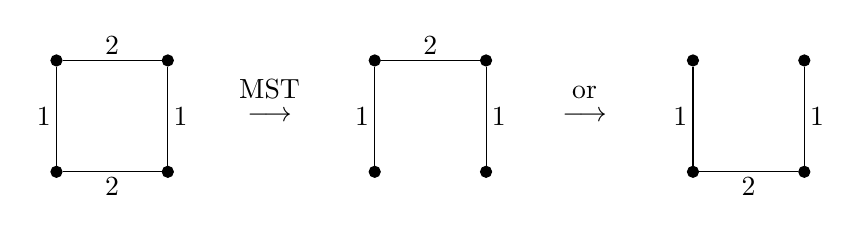
\begin{tikzpicture}[black/.style={circle,draw,fill=black,inner sep=0pt, minimum width=4pt}]
	\foreach \x in {45,135,225,315}
		\node[black] at (\x:1) (\x) {};
	\draw (45) -- (135) node [midway,label=above:{2},yshift=-5] {};
	\draw (135) -- (225) node [midway,label=left:{1},xshift=5] {};
	\draw (225) -- (315) node [midway,label=below:{2},yshift=5] {};
	\draw (315) -- (45) node [midway,label=right:{1},xshift=-5] {};


	\draw node at (2,0) {$\longrightarrow$};
	\draw[above,yshift=3] node at (2,0) {MST};


	\foreach \x in {45,135,225,315}
		\node[black,xshift=115] at (\x:1) (\x) {};
	\draw (45) -- (135) node [midway,label=above:{2},yshift=-5] {};
	\draw (135) -- (225) node [midway,label=left:{1},xshift=5] {};
	% \draw (225) -- (315) node [midway,label=below:{2},yshift=5] {};
	\draw (315) -- (45) node [midway,label=right:{1},xshift=-5] {};


	\draw node at (6,0) {$\longrightarrow$};
	\draw[above,yshift=3] node at (6,0) {or};


	\foreach \x in {45,135,225,315}
		\node[black,xshift=230] at (\x:1) (\x) {};
	% \draw (45) -- (135) node [midway,label=above:{2},yshift=-5] {};
	\draw (135) -- (225) node [midway,label=left:{1},xshift=5] {};
	\draw (225) -- (315) node [midway,label=below:{2},yshift=5] {};
	\draw (315) -- (45) node [midway,label=right:{1},xshift=-5] {};
\end{tikzpicture}
